\documentclass[12pt]{beamer}
\geometry{paper=a6paper,landscape}

\usetheme{default}% I recommend
% \or\usetheme{Singapore}
% \or\usetheme{Boadilla}
% \or\usetheme{Pittsburgh}
% \or\usetheme{Madrid}
% \or\usetheme{Warsaw} % common choice, but often poor
% \fi
\usepackage{changepage}
\usepackage{minted}
\usepackage{graphicx,pgfplots,parskip}
\usepackage{listings}
\usepackage{semantic}
\usepackage[utf8]{inputenc}
\usepackage[T1]{fontenc}
\usepackage{microtype}
\usepackage{amsmath}
\usepackage{amssymb}
\usepackage{ifthen}
\newcommand\hmmax{0} % default 3
% \newcommand\bmmax{0} % default 4
% \usepackage{bm}
\usepackage{stmaryrd}
\usepackage{proof}
\usepackage{graphicx}
\usepackage[export]{adjustbox}
\usepackage{listings}
\usepackage{tikz}
\usepackage{semantic}
\usepackage{setspace}
\usepackage{wrapfig}
\usepackage{color}
\usepackage{caption}
\usepackage{subcaption}
\usepackage{esvect}
\usepackage{tikz}
\usepackage{booktabs} %% http://ctan.org/pkg/booktabs
\usepackage{wasysym}
\usepackage{array,multirow}
\usepackage{balance}
\usepackage[backend=bibtex, style=authoryear-comp]{biblatex}

\title{Haskell DSL for Automatic Differentiation at Scale}
\subtitle{based on Conal Elliott's paper: Simple Essence of Automatic Differentiation}
\author{Deyaaeldeen Almahallawi\\
  Bloomberg L.P., Indiana University}

\date{August 2019}

\begin{document}

\begin{frame}
\maketitle
\end{frame}

\begin{frame}{Outline}
\tableofcontents
\end{frame}

\section{Introduction}

\begin{frame}{Problem Statement}

Finite-difference approximation cons:
\begin{itemize}
\item requires at least two runs for each argument
\item multiple runs might be needed to calibrate $\epsilon$
\end{itemize}
\pause
Automatic Differentiation pros:
\begin{itemize}
\item exact results
\item little computational overhead
\end{itemize}
\pause
Existing AD libraries cons:
\begin{itemize}
\item involves mutation, graph construction and traversal, and tapes
  (Wengert lists)
\item parallelization could be challenging
\item do not scale well to arbitrarily higher dimensions (different
  chain rules)
\end{itemize}
\end{frame}

\begin{frame}{What is a derivative}

\begin{equation*}
  f'(x)=\lim_{\epsilon \to 0} \frac{f(x+\epsilon) - f(x)}{\epsilon}
\end{equation*}
\pause
\begin{equation*}
  \lim_{\epsilon \to 0} \frac{f(x+\epsilon) - f(x)}{\epsilon}-f'(x)=0
\end{equation*}
\pause
\begin{equation*}
  \lim_{\epsilon \to 0} \frac{f(x+\epsilon) - (f(x) + (\epsilon . f'(x)))}{\epsilon}=0
\end{equation*}
\pause
\begin{equation*}
  \lim_{\epsilon \to 0} \frac{\left\|f(x+\epsilon) - (f(x) + (\epsilon . f'(x)))\right\|}{\left\|\epsilon\right\|}=0
\end{equation*}
\end{frame}

\begin{frame}[fragile]{Derivatives are linear maps}

\begin{minted}[escapeinside=||,mathescape=true]{haskell}
  D :: (a -> b) -> (a -> (a :-* b))
  D (g |$\circ$| f) a = D g (f a) |$\circ$| D f a
\end{minted}
  \pause
  Example:
\begin{minted}[escapeinside=||,mathescape=true]{haskell}
  D :: (|$\mathbb{R}$| -> |$\mathbb{R}$|) -> (|$\mathbb{R}$| -> (|$\mathbb{R}$| :-* |$\mathbb{R}$|))
  D (sin |$\circ$| cos) a = D sin (cos a) |$\circ$| D cos a
\end{minted}
\end{frame}

\begin{frame}[fragile]{Chain rule is linear map composition}
\begin{minted}[escapeinside=||,mathescape=true]{haskell}
  D|$^{+}$| :: (a -> b) -> (a -> (b, (a :-* b)))
  D|$^{+}$| f a = (f a, D f a)
\end{minted}

\begin{minted}[escapeinside=||,mathescape=true]{haskell}
  D|$^{+}$| (g |$\circ$| f) a = let (b, f') = D|$^{+}$| f a
                     (c, g') = D|$^{+}$| g b
                 in (c, g' |$\circ$| f')
\end{minted}
\end{frame}

\begin{frame}[fragile]{Linear functions}
  Linear maps properties:
  \begin{align*}
    f(a + a') &= f(a) + f(a')\\
    f(s . a) &= s . f(a) 
  \end{align*}

\pause{}
How to differentiate linear maps:
\begin{minted}[escapeinside=||,mathescape=true]{haskell}
                      D f a = f
\end{minted}
\pause
\begin{minted}[escapeinside=||,mathescape=true]{haskell}
                     D|$^{+}$| f a = (f a, f)
\end{minted}
\end{frame}

\begin{frame}[fragile]{Abstract algebra for functions}
\begin{minted}[escapeinside=||,mathescape=true]{haskell}
class Category k where
  id  :: a `k` a
  (|$\circ$|) :: (b `k` c) -> (a `k` b) -> (a `k` c)

class Category k => CartesianCat k where
  exl :: (a, b) `k` a
  exr :: (a, b) `k` b
  dup :: a `k` (a, a)
\end{minted}
\end{frame}

\begin{frame}[fragile]{Category of functions}
\begin{minted}[escapeinside=||,mathescape=true]{haskell}
instance Category (->) where
  id  = id
  (|$\circ$|) = (|$\circ$|)

instance CartesianCat (->) where
  exl = fst
  exr = snd
  dup a = (a, a)
\end{minted}
\end{frame}

\section{Automatic Differentiation}

\begin{frame}{Outline}
\tableofcontents[currentsection]
\end{frame}

\begin{frame}[fragile]{Automatic Differentiation}
\begin{minted}[escapeinside=||,mathescape=true]{haskell}
type a :-* b = a -> b
newtype D a b = D {unD :: a -> (b, a :-* b)}

linearD :: (a -> b) -> D a b
linearD f = D (\a -> (f a, f))

instance Category D where
  id = linearD id
  (|$\circ$|) (D g) (D f) = D (\a -> let (b,f') = f a
                                 (c,g') = g b
                             in (c, g' |$\circ$| f'))
                             
instance CartesianCat D where
  exl = linearD exl
  exr = linearD exr
  dup = linearD dup
\end{minted}
\end{frame}

\begin{frame}[fragile]{Automatic Differentiation}
  
\begin{minted}[escapeinside=||,mathescape=true]{haskell}

(&&&) :: Category k => (a `k` c) -> (a `k` d) -> (a `k` (c, d))
  
instance (AdditiveGroup s, Num s) => NumCat D s where
  addC    = linearD addC
  negateC = linearD negateC
  mulC    = D (mulC &&& \ (u,v) -> \(du,dv) -> u*dv + v*du)
\end{minted}
\end{frame}

\begin{frame}[fragile]{Example}

\begin{adjustwidth}{-1.8em}{-1.8em}
\begin{minted}[escapeinside=||,mathescape=true]{haskell}

sqr :: (Category k, Num a) => a `k` a
sqr = mulC |$\circ$| (id &&& id)

sqr :: Num a => a -> a
sqr a = a * a

magSqr :: (Category k, Num a) => (a, a) `k` a
magSqr = addC |$\circ$| ((mulC |$\circ$| (exl &&& exl)) &&& (mulC |$\circ$| (exr &&& exr)))

magSqr :: Num a => (a, a) -> a
magSqr (a, b) = sqr a + sqr b
  
\end{minted}
\end{adjustwidth}
\end{frame}

\begin{frame}[fragile]{Visualization}
% \begin{adjustwidth}{-1.8em}{-1.8em}
  \begin{center}
    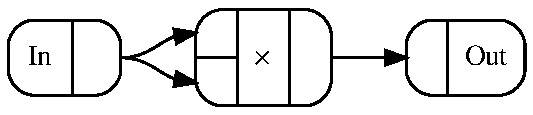
\includegraphics[width=4in]{figures/sqr}
  \end{center}
  \vspace{1cm}
  \begin{center}
    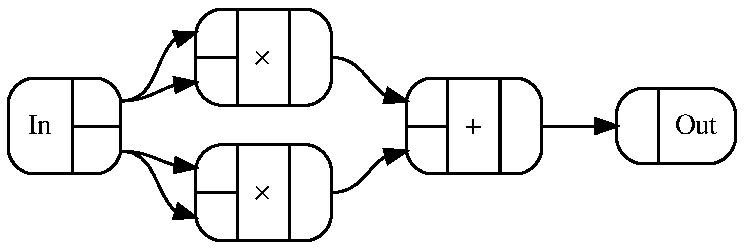
\includegraphics[width=4in]{figures/magSqr}
  \end{center}
% \end{adjustwidth}
\end{frame}

\begin{frame}[fragile]{Derivative Visualization}
  \begin{center}
    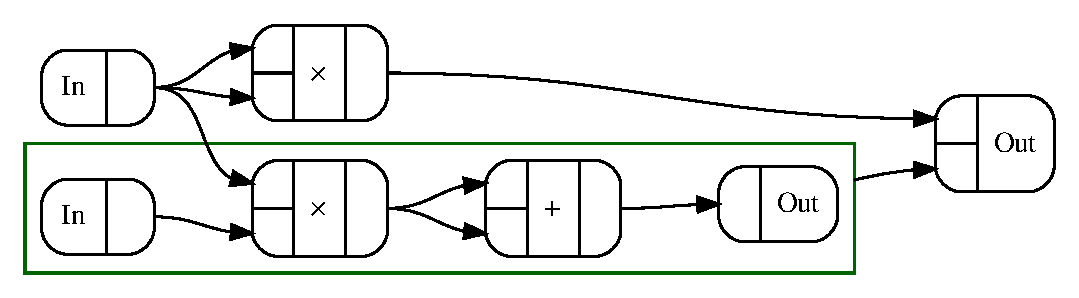
\includegraphics[width=4in]{figures/sqr-adf}
  \end{center}
  \vspace{1cm}
  \begin{center}
    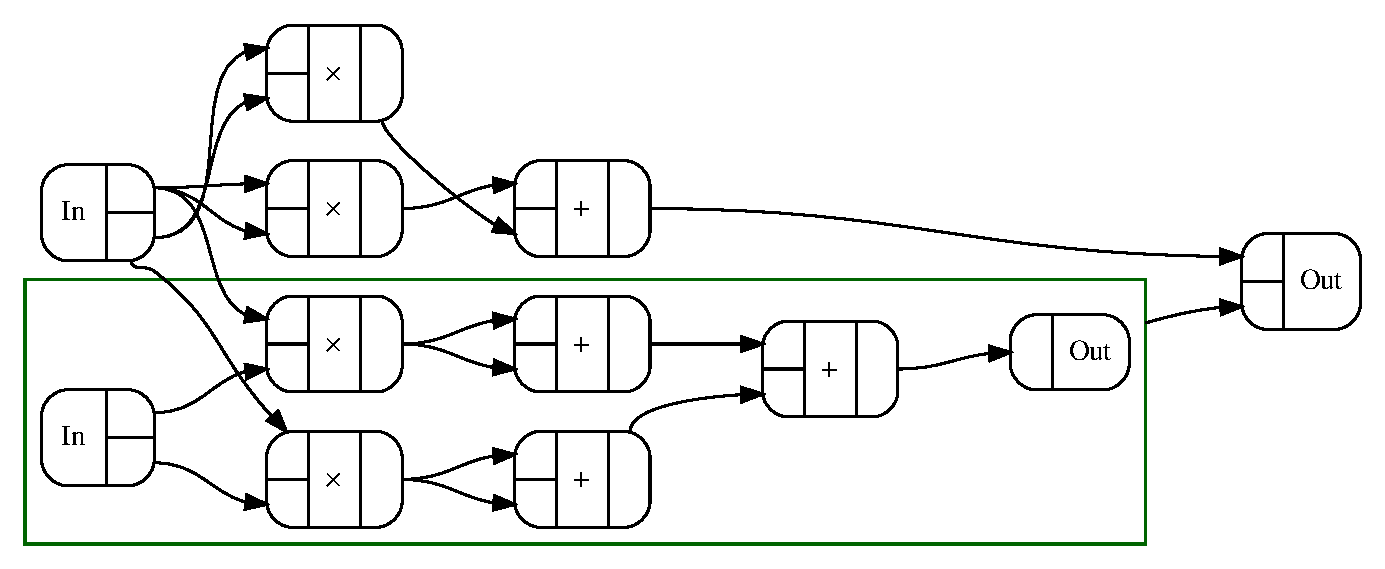
\includegraphics[width=4in]{figures/magSqr-adf}
  \end{center}
\end{frame}

\begin{frame}[fragile]{Sharing Example}

\begin{adjustwidth}{-1.8em}{-1.8em}
\begin{minted}[escapeinside=||,mathescape=true]{haskell}

cosSinProd :: (a, a) `k` (a, a)
cosSinProd = (cosC &&& sinC) |$\circ$| mulC
\end{minted}
\end{adjustwidth}

\begin{center}
  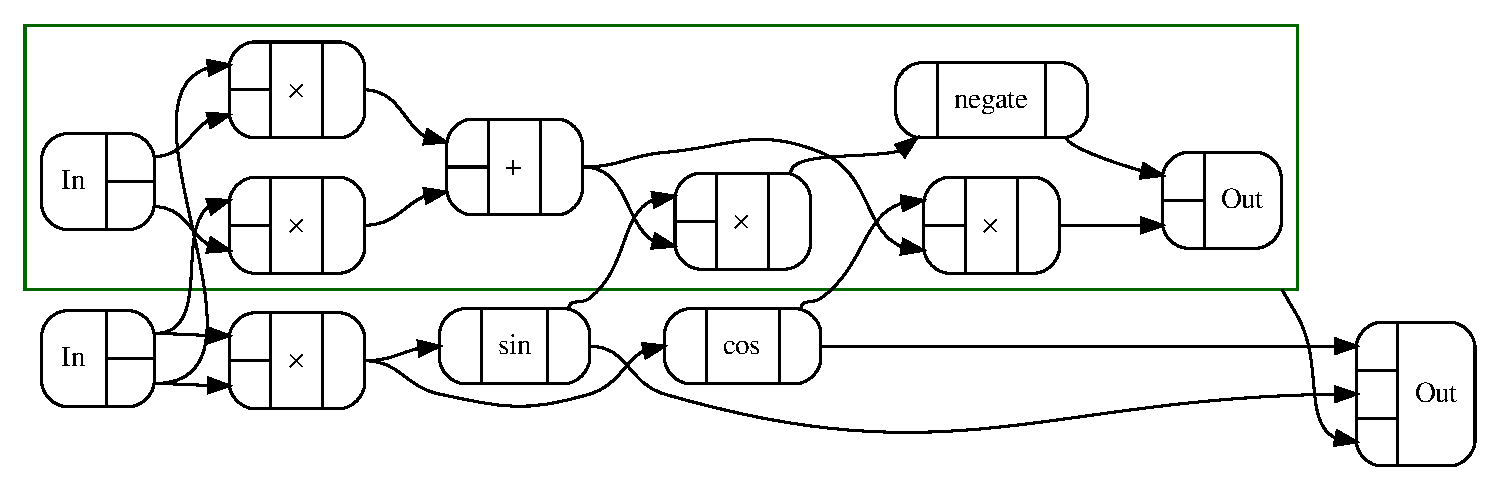
\includegraphics[width=4in]{figures/cosSinProd-adf}
\end{center}
\end{frame}


\section{Generalization}

\begin{frame}{Outline}
\tableofcontents[currentsection]
\end{frame}

\begin{frame}[fragile]{Generalized Automatic Differentiation}
\begin{minted}[escapeinside=||,mathescape=true]{haskell}
newtype D k a b = D {unD :: a -> (b, a `k` b)}

linearD :: Category k => (a -> b) -> (a `k` b) -> D k a b
linearD f f' = D (\a -> (f a, f'))

instance Category k => Category (D k) where
  id = linearD id id
  (|$\circ$|) (D g) (D f) = D (\a -> let (b,f') = f a
                                 (c,g') = g b
                             in (c, g' |$\circ$| f'))
                             
instance CartesianCat k => CartesianCat (D k) where
  exl = linearD exl exl
  exr = linearD exr exr
  dup = linearD dup dup
\end{minted}
\end{frame}

\begin{frame}[fragile]{Generalized Automatic Differentiation}
  \begin{minted}[escapeinside=||,mathescape=true]{haskell}
instance (Category k, Num s) => NumCat (GD k) s where
  addC    = linearD addC jam
  negateC = linearD negateC (scale (-1))
  mulC    = D (mulC &&& \ (u, v) -> scale v +++ scale u)

class Category k => CocartesianCat k where
  inl :: a `k` (a, b)
  inr :: b `k` (a, b)
  jam :: (a, a) `k` a

class Category k => ScalarCat k a where
  scale :: a -> a `k` a

(+++) :: (c `k` a) -> (d `k` a) -> ((c, d) `k` a)
f +++ g = jam |$\circ$| (f *** g)
\end{minted}
\end{frame}

\begin{frame}[fragile]{Linear Transformations as Functions}
  \begin{minted}[escapeinside=||,mathescape=true]{haskell}

newtype a -+> b = AddFun {unAddFun :: a -> b}

deriving instance AdditiveGroup b => AdditiveGroup (a -+> b)

instance Category (-+>) where
  id = AddFun id
  AddFun g |$\circ$| AddFun f = AddFun (g |$\circ$| f)

deriving instance CartesianCat (-+>)

instance CocartesianCat (-+>) where
  inl = AddFun (,zero)
  inr = AddFun (zero,)
  jam = AddFun (uncurry (^+^))

instance Num s => ScalarCat (-+>) s where
  scale s = AddFun (s *)

\end{minted}
\end{frame}

\section{Reverse-mode}

\begin{frame}{Outline}
\tableofcontents[currentsection]
\end{frame}

\begin{frame}[fragile]{RAD by Left Association}
  \begin{minted}[escapeinside=||,mathescape=true]{haskell}

newtype Cont k r a b = Cont {runCont :: b `k` r -> a `k` r}

instance Category (Cont k r) where
  id = Cont id
  (|$\circ$|) = inAbst2 (flip (|$\circ$|))

instance CartesianCat k => CartesianCat (Cont k r) where
  exl = Cont (+++ zeroC)
  exr = Cont (zeroC +++)
  dup = Cont (uncurry plusC |$\circ$| unjoin)

instance (CocartesianCat k) => CocartesianCat (Cont k r) where
  inl = Cont (exl |$\circ$| unjoin)
  inr = Cont (exr |$\circ$| unjoin)
  jam = Cont (join |$\circ$| dup)

\end{minted}
\end{frame}

\begin{frame}[fragile]{RAD Specialization to Backpropagation}
  \begin{minted}[escapeinside=||,mathescape=true]{haskell}

newtype Dual k a b = Dual {unDual :: b `k` a}

instance Category k => Category (Dual k) where
  id = Dual id
  (|$\circ$|) = inAbst2 (flip (|$\circ$|))

instance CocartesianCat k => CartesianCat (Dual k) where
  exl = Dual inl
  exr = Dual inr
  dup = Dual jam

instance CartesianCat k => CocartesianCat (Dual k) where
  inl = Dual exl
  inr = Dual exr
  jam = Dual dup

instance ScalarCat k s => ScalarCat (Dual k) s where
  scale s = Dual (scale s)

\end{minted}
\end{frame}

\section{Contributions}

\begin{frame}{Outline}
\tableofcontents[currentsection]
\end{frame}

\begin{frame}{Contributions}
  \begin{itemize}
  \item implemented the presented DSL and multiple representations of
    linear maps
  \item added support for new constructs: more primitives and
    conditionals
  \item wrote a collection of programs for predicting option prices
    (Black-Scholes, monte carlo for european and asian options)
  \item understanding different performance trade-offs
  \item differentiated code can be linked with existing C code
  \item added testing and benchmarking infrastructure
  \end{itemize}
\end{frame}

\section{Performance}

\begin{frame}{Outline}
\tableofcontents[currentsection]
\end{frame}

\begin{frame}[fragile]{Monte-Carlo Structure}
\begin{adjustwidth}{-1.8em}{-1.8em}
\resizebox{14cm}{7cm}{%
\begin{tikzpicture}[level/.style={sibling distance=60mm/#1}]
\node [circle,draw] (z){$n$}
  child {node [circle,draw] (a) {$p_1$}
    child {node {$\vdots$}}
  }
  child {node [circle,draw] (b) {$p_2$}
    child {node {$\vdots$}}
  }
  child {node [circle,draw] (c) {$p_i$}
    child {node [circle,draw] (d) {$t_1$}
      child {node (e){$\vdots$}
        child {node [circle,draw] (f) {$t_i$}
          child {node {$\vdots$}
            child {node [circle, draw] (g) {$t_m$}
              child {node [circle, draw] (h) {payoff}}
            }
        }
      }
    }
  }
}
child {node [circle,draw] (i) {$p_{n-1}$}
    child {node {$\vdots$}}
  }
child {node [circle,draw] (j) {$p_n$}
  child {node {$\vdots$}}
};
% \path (a) -- (j) node [midway] {+};
% \path (b) -- (g) node [midway] {+};
% \path (k) -- (l) node [midway] {+};
% \path (k) -- (g) node [midway] {+};
% \path (d) -- (e) node [midway] {+};
% \path (o) -- (p) node [midway] {+};
% \path (o) -- (e) node (x) [midway] {$\cdots$}
%   child [grow=down] {
%     node (y) {$O\left(\displaystyle\sum_{i = 0}^k 2^i \cdot \frac{n}{2^i}\right)$}
%     edge from parent[draw=none]
%   };
% \path (q) -- (r) node [midway] {+};
% \path (s) -- (r) node [midway] {+};
% \path (s) -- (t) node [midway] {+};
% \path (s) -- (l) node [midway] {=};
% \path (t) -- (u) node [midway] {+};
% \path (z) -- (u) node [midway] {=};
% \path (j) -- (t) node [midway] {=};
% % \path (y) -- (x) node [midway] {$\Downarrow$};
% % \path (v) -- (y)
% %   node (w) [midway] {$O\left(\displaystyle\sum_{i = 0}^k n\right) = O(k \cdot n)$};
% \path (q) -- (v) node [midway] {=};
% % \path (e) -- (x) node [midway] {+};
% % \path (o) -- (x) node [midway] {+};
% % \path (y) -- (w) node [midway] {$=$};
% % \path (v) -- (w) node [midway] {$\Leftrightarrow$};
% \path (r) -- (c) node [midway] {$\cdots$};
\end{tikzpicture}
}
\end{adjustwidth}
\end{frame}

\begin{frame}{Performance}
\begin{adjustwidth}{-1.8em}{-1.8em}
  \begin{center}
    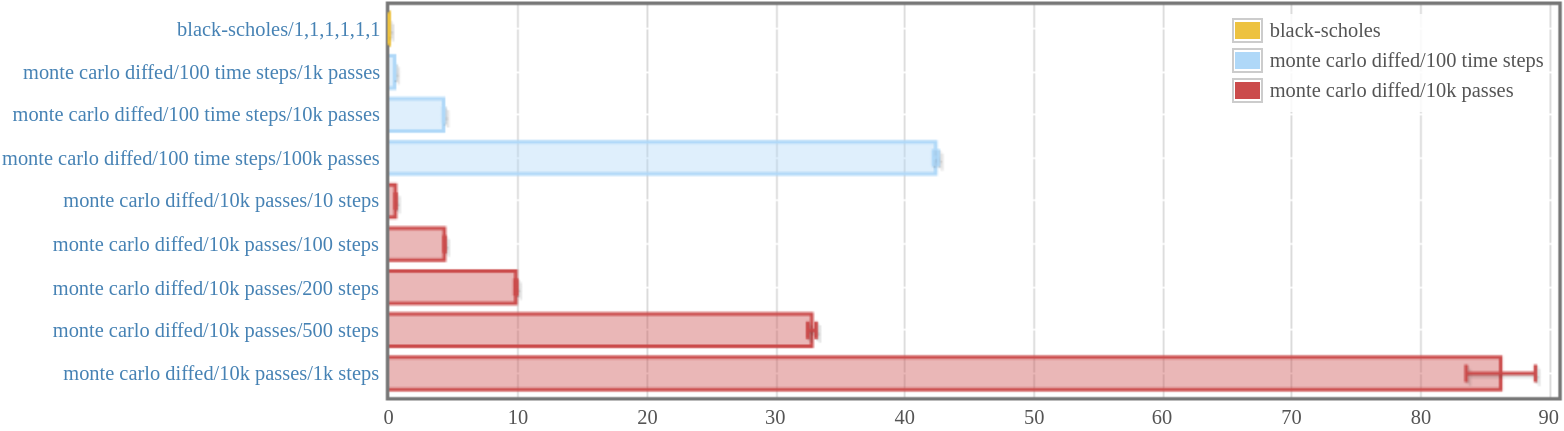
\includegraphics[width=5.5in]{figures/overview}
  \end{center}  
\end{adjustwidth}
\end{frame}

\begin{frame}{Performance}
\begin{adjustwidth}{-1.8em}{-1.8em}
  \begin{center}
    \begin{itemize}
    \item Forward-mode derivative runtime / Primal runtime = $2.75$
    \item Reverse-mode derivative runtime / Primal runtime = $8.75$
    \item Forward-mode derivative runtime / Finite-difference
      approximation runtime for 1 greek = $1.3$
    \item Reverse-mode derivative runtime / Finite-difference
      approximation runtime for all greeks = $1.1$
    \end{itemize}
  \end{center}  
\end{adjustwidth}
\end{frame}

\section{Conclusion}

\begin{frame}{Outline}
\tableofcontents[currentsection]
\end{frame}

\frame{
\frametitle{Conclusion}

\begin{itemize}
\item
  -- is Automatic Differentiation feasible for monte-carlo simulations
  with huge number of simulation passes? yes,~40s for 100k passes \\
  and with large number of time steps? yes,~80s for 1k steps \\
  -- is Automatic Differentiation memory efficient? yes,~1MB max \\
  -- can Automatic Differentiation be integrated seamlessly with existing
  code base without compile-time blow-up? yes, it is distributed as a
  shared library

\item Next steps:\\
  -- custom compilation\\
  -- taking advantage of parallel execution\\
  -- support more language constructs \\
  -- provide a user-friendly front-end that compiles to categorical
  primitives
\end{itemize}

\begin{center}
  \url{https://bbgithub.dev.bloomberg.com/dalmahallawi/autodiff}
\end{center}

}
  
\end{document}

%%% Local Variables:
%%% mode: latex
%%% TeX-master: t
%%% End:
%%% Local Variables:
%%% mode: latex
%%% End:
